% -*- TeX-master: "main" -*-

\section{Package syntax and semantics}
\label{syntax}

This section contains a definition of the syntax and semantics of the Required Element package for \sbmlthreecore.  

% --------------------------------------------------------------------------
\subsection{Namespace URI and other declarations necessary for using this package}
\label{xml-namespace}

Every SBML Level~3 package is identified uniquely by an XML namespace URI.  For an SBML document to be able to use a given Level~3 package, it must declare the use of that package by referencing its URI.  The following is the namespace URI for this version of the Required Elements package for \sbmlthreecore:
\begin{center}
\uri{http://www.sbml.org/sbml/level3/version1/req/version1}
\end{center}

In addition, SBML documents using a given package must indicate whether understanding the package is required for complete mathematical interpretation of a model.  This is done using the attribute \token{required} on the \token{<sbml>} element in the SBML document.  For the Required Elements package, the value of this attribute must be \val{false}, because while the Required Elements package is designed to clarify how other packages change the mathematical meaning of the model, it cannot itself do so.

The following fragment illustrates the beginning of a typical SBML model using \sbmlthreecore and this version of the Required Elements package:

\begin{example}
<?xml version="1.0" encoding="UTF-8"?>
<sbml xmlns="http://www.sbml.org/sbml/level3/version1/core" level="3" version="1"
      xmlns:req="http://www.sbml.org/sbml/level3/version1/req/version1" req:required="false">
\end{example}


\subsection{Primitive data types}
\label{new-primitive-types}

The Required Elements package uses three of the data types described in Section~3.1 of the \sbmlthreecore specification, specifically \primtype{SId}, \primtype{string} and \primtype{boolean}.  The package does not define any new types.


\begin{figure}[bh]
  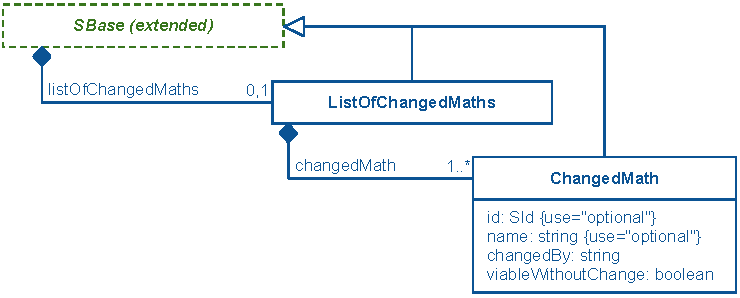
\includegraphics{figs/extended-sbase-req-uml}
  \vspace*{-0.0em}
  \caption{The definition of the extended \SBase class, and the new \ListOfChangedMaths and \ChangedMath classes.}
  \label{extended-sbase-uml}
\end{figure}

\subsection{The extended \class{SBase} class}
\label{extended-sbase-class}

As mentioned above, this package's reason for being is to define an optional child of the SBML Level~3 \SBase class.  \fig{extended-sbase-uml} provides the definition of this \SBase extension, and its optional \ChangedMath children.  These children are added to \SBase instead of to those elements that have math in them (such as \InitialAssignment, \KineticLaw, etc.) or that have mathematical meaning (such as \Parameter or \Species) because this approach allows other SBML Level~3 packages to define new elements with mathematics which may, in turn, be overridden by other packages.

\subsection{The \class{ListOfChangedMaths} class}
\label{listofchangedMaths-class}

As is standard in SBML specifications, any time more than one child of the same class is to be added to an element, a 'ListOf' that element is provided to store them, and to collect annotations about the list itself.  The child 'listOfChangedMaths' on SBase is optional, but if present, must contain one or more 'changedMath' children.

\subsection{The \class{ChangedMath} class}
\label{changedMath-class}

The \ChangedMath class defines an element, one or more of which may be added to any SBML element that either has mathematical meaning, or that contains a \Math child.  In SBML Level~3 Core, the former group includes the classes \Compartment, \Parameter, \Reaction, \Species, and \SpeciesReference, and the latter group includes the classes \Constraint, \Delay, \EventAssignment, \FunctionDefinition, \InitialAssignment, \KineticLaw, \Priority, \Rule, and \Trigger.  \Event elements do not have any direct \Math children, but do indirectly, and may thus be given a \ChangedMath child.  Packages that introduce elements that have mathematical meaning and/or that contain \Math children may also be extended through the addition of a \ChangedMath child, when some other package changes that element's mathematical interpretation.

Elements with mathematical meaning may have a \ChangedMath child when a package alters the value or meaning of that symbol.  As an example, a \Submodel from the Hierarchical Model Composition package may contain an \Event or \Rule that assigns new values to a parameter.  Because an interpreter that did not understand submodels would not catch this change, the Hierarchical Model Composition package can be seen to change the math of that element, and it would be appropriate to denote this by adding a \ChangedMath child to the affected parameter.

Similarly, models that use the proposed Spatial Processes package can change the meaning of a \Compartment by turning it into a bounded object with an size implied by those boundaries (and how they change over time), instead of using the element's \token{size} attribute.  Spatial Processes elements may also change a \Species to be spatially defined, and therefore represent different values depending on what coordinates in space are under consideration.  Affected compartments and species could be given \ChangedMath children to denote this fact.

Elements with \Math children may also be changed by the addition of package elements.  Some packages may instruct the modeler to disregard the \Math and to use some other construct instead.  For example, the proposed Distrubutions package adds a new child to \FunctionDefinition, which replaces the old mathematics with a new set of mathematics returning a draw from a random distribution (something impossible with \Math).

Each package may define for itself when it would be appropriate or necessary, given the package's structure, to add a \ChangedMath element to something.  If no such definition exists, a user may add \ChangedMath elements where they understand the math to be changing.

For packages with no such rules, the addition of \ChangedMath children cannot be guaranteed to be normative, that is, software that understands the Required Elements package, but which does not understand some other package flagged \token{required}=\val{true} will not be able to assert that every element with altered mathematics has been given a \ChangedMath child.  However, a package may define its own validation rules in conjunction with this Required Elements package, and a user may then be able to guarantee that any affected element has been denoted as such.

Note that a \ChangedMath element should be added to the model component that is directly affected only, and not on a component that is indirectly affected by the changed mathematics.  For example, if a model contains a \FunctionDefinition object whose mathematics are extended by the SBML Level~3 package for Distributions, and elsewhere in the model there is an \InitialAssignment object that uses that function, a \ChangedMath child should be added only to the \FunctionDefinition object and not the \InitialAssignment nor on the element that assigns to, because the latter are only indirectly affected, through processes understood without reference to package definitions.

Multiple packages may affect the mathematics of the same object in different ways.  For example, a construct from the Spatial Process package could change a \Species to be spatially defined, and that same model may have a \Submodel from the Hierarchical Model Composition package which contains a \Reaction that affects that \Species.  In that case, the \Species would have two \ChangedMath children, one for each package that affects it.

Since \ChangedMath itself has no mathematical meaning and no child \Math object, it may not itself have a \ChangedMath child.

\subsubsection{The \fixttspace\tokenNC{id} and \fixttspace\tokenNC{name} attributes}
\label{idname-attributes}

The optional \token{id} attribute on the \ChangedMath object class serves to provide a way to identify the element.  The attribute takes a value of type \primtype{SId}.  Note that this identifier carries no mathematical interpretation and cannot be used in mathematical formulas in a model.  \ChangedMath also has an optional \token{name} attribute, of type \primtype{string}.  The \token{name} attribute may be used in the same manner as other \token{name} attributes on \sbmlthreecore objects; please see Section~3.3.2 of the \sbmlthreecore specification for more information.


\subsubsection{The \fixttspace\tokenNC{changedBy} attribute}
\label{attribute-changedBy}

The \token{changedBy} attribute is required, and is of type \token{string}.  The attribute must be set to the namespace URI of the SBML Level~3 package that redefines or alters the mathematical semantics of the parent object.  In other words, if the mathematical semantics of a given component \emph{C} in a model is changed by the use of a Level~3 package \emph{P}, then \emph{C} can be given a \ChangedMath child, and its attribute \token{changedBy} should be \emph{P}'s namespace URI.  The examples below will make this more clear.

Valid values for the \token{changedBy} token include the namespace URI for any SBML L3 package flagged \token{required} =\val{true}.  If there are no such packages present in the SBML Document, there is no valid value for the \token{changedBy} attribute, and therefore no \ChangedMath element may appear in the document.

No two child \ChangedMath elements of any single \SBase object may have the same \token{changedBy} value.  


\subsubsection{The \fixttspace\tokenNC{viableWithoutChange} attribute}
\label{attribute-absenceleavesalternative}

The \token{viableWithoutChange} attribute is required, and is of type \token{boolean}.  The attribute should be used to indicate whether an interpreter that does not understand the package from the \token{changedBy} attribute would have an interpretable version of the mathematics for the given component in a model.  This can be established using two criteria:  ``Complete'' and ''Workable''.  Obviously, if the math being interpreted is incomplete, the \token{viableWithoutChange} attribute must be \val{false}.  If the math is complete, then whether the solution is ``workable'' requires a judgement call on the part of the modeler: if the modeler feels that the alternative version makes sense in an alternative context, they may set the attribute value to \val{true}; conversely, if they feel that the resulting model component makes no sense, even if technically ``complete'', then they should set the attribute value to \val{false}.

When two different packages alter the mathematical interpretation of an \SBase object in different ways, and two corresponding \ChangedMath elements are added, each should consider whether the aspect of the change that package is responsible for has an alternative, irrespective of how the other package affects the element.  In our above example where both the Spatial Processes and the Hierarchical Model Composition package affected the same \Species, the \ChangedMath element for the Spatial Processes package may have its \token{viableWithoutChange} attribute set to \val{true} if an alternate framework without Spatial Processes constructs is present (even if spread across multiple \Submodel elements from the Hierarchical Model Composition package).  Conversely, if the \Reaction that affects the \Species is in a \Submodel, the corresponding \token{viableWithoutChange} for that package should be set to \val{false} if that \Reaction is considered vital to the understanding and interpertation of the model.


\subsection{Additional considerations}

The Required Elements package is not, itself, required (that is, models that use it must set \token{required}=\val{false} for its namespace when using it) because it, in and of itself, does not change any mathematical semantics.  However, it is intended to be used by other required packages, which may in turn make the use of this package in certain contexts defined in those package specifications. 
